%
% File acl2013.tex
%
% Contact  navigli@di.uniroma1.it
%%
%% Based on the style files for ACL-2012, which were, in turn,
%% based on the style files for ACL-2011, which were, in turn, 
%% based on the style files for ACL-2010, which were, in turn, 
%% based on the style files for ACL-IJCNLP-2009, which were, in turn,
%% based on the style files for EACL-2009 and IJCNLP-2008...

%% Based on the style files for EACL 2006 by 
%%e.agirre@ehu.es or Sergi.Balari@uab.es
%% and that of ACL 08 by Joakim Nivre and Noah Smith

\documentclass[11pt]{article}
\usepackage{acl2013}
\usepackage{times}
\usepackage{url}
\usepackage{latexsym}
\usepackage{graphicx}  
\graphicspath{ {img/} }
\usepackage{listings}
\usepackage{color}
\definecolor{lightgray}{rgb}{.9,.9,.9}
\definecolor{darkgray}{rgb}{.4,.4,.4}
\definecolor{purple}{rgb}{0.65, 0.12, 0.82}

\lstdefinelanguage{JavaScript}{
  keywords={typeof, new, true, false, catch, function, return, null, catch, switch, var, if, in, while, do, else, case, break},
  keywordstyle=\color{blue}\bfseries,
  ndkeywords={class, export, boolean, throw, implements, import, this},
  ndkeywordstyle=\color{darkgray}\bfseries,
  identifierstyle=\color{black},
  sensitive=false,
  comment=[l]{//},
  morecomment=[s]{/*}{*/},
  commentstyle=\color{purple}\ttfamily,
  stringstyle=\color{red}\ttfamily,
  morestring=[b]',
  morestring=[b]"
}

\lstset{
   language=JavaScript,
   backgroundcolor=\color{lightgray},
   extendedchars=true,
   basicstyle=\footnotesize\ttfamily,
   showstringspaces=false,
   showspaces=false,
   numbers=left,
   numberstyle=\footnotesize,
   numbersep=9pt,
   tabsize=2,
   breaklines=true,
   showtabs=false,
   captionpos=b
}

%\setlength\titlebox{6.5cm}    % You can expand the title box if you
% really have to

\title{JavaScript Test-Driven Development with Jasmine and Karma}

\author{Cedric Takongmo \\
{\tt cedric.takongmo@mni.thm.de}}

\date{}

\begin{document}
\maketitle
\begin{abstract}
Get a concise introduction to Jasmine, the popular testing framework for JavaScript. This document shows you how to write unit tests with Jasmine that automatically check for bugs in your application using the Test-Driven development pattern and the Karma test runner. After you get an overview of test-driven development, learn how to write specifications for individual components, and then use those specs to test the code you write. Write useful specs by determining what you need to test and what you don’t. Test the behavior of new and existing code against the specs you create. Apply Jasmine matchers and discover how to build your own. Organize code suites into groups and subgroups as your code becomes more complex. Use a Jasmine spy in place of a function or an object and learn why it’s valuable.

\end{abstract}

\section{Credits}

This document has been wrote on the basis of some external Internet links and a presentation of Christopher Bartling about JavaScript tests with Jasmine and Karma. The statistics to illustrate the importance of JavaScript today come from studies of diverse companies like TIOBE software. A detailed presentation of the Jasmine library was inspired by the online documentation on the official Jasmine website. 

\section{Motivation for Javascript TDD}

Today, Javascript is growing in popularity and will continue to grow. As show in the Abbildung 1, from 1996 to 2016, JavaScript is from the 23th to the 7th position of the most used programming languages. JavaScript is also used all over the place, and is used even with every backend language. This programming language is also the most commonly used in frontend development to dynamically give more user experience to web applications. JS-libraries are used for the development of web and mobile applications with JQuery Mobile/PhoneGap. Famous libraries like Angular.js, jQuery, Node.js, React and various others tools inherit JavaScript. Some hardware engineer are using JavaScript to do embedded programming so that JavaScript can be used for the direct communication with the outside world by using MicroControllers and other electronics related stuff, although this is definitely less common at the moment. This is why JavaScript is such a good language to learn.

A software product has to be considered like every other commercial product and it quality must be tested. This is also valid for javaScript Software. In the software engineering, we are talking about Code Quality. Code quality is a loose approximation of how long-term useful and long-term maintainable the code is. If the Code is thrown away tomorrow is mean that this Code has a Low quality. High quality Code is being carried over from product to product, developed further, maybe even open sourced after establishing is value. The software quality is defined with a clear and understandable design and implementation and also well defined interfaces. Good Code is ease to build and use and have to be extensible. The minimum extra dependencies and the good documentation are very important criteria for Software Quality. One off he most important criteria are the tests: Unit, integration, and functional/acceptance testing.

In this context of Code Quality and Unit Testing in JavaScript, Test-driven development (TDD) is the new trend. TDD is a new way to software development which combines test-first development where you write a test before you write just enough production code to fulfill that test and refactoring. What is the primary goal of TDD? One view is the goal of TDD is specification and not validation (Martin, Newkirk, and Kess 2003). In other words, it’s one way to think through your requirements or design before your write your functional code (implying that TDD is both an important agile requirements and agile design technique). Another view is that TDD is a programming technique. As Ron Jeffries likes to say, the goal of TDD is to write clean code that works. I think that there is merit in both arguments, although I lean towards the specification view, but I leave it for you to decide. 

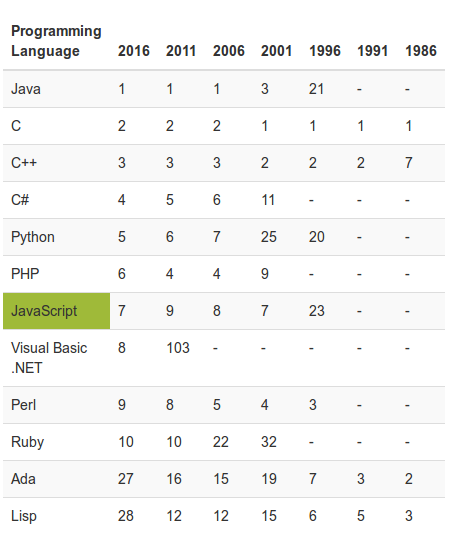
\includegraphics[scale=0.3]{Motivation.png}
\section{Test-driven development cycle}
TDD can be described, as explained in, with this simple formula: TDD = The steps of test first development (TFD) + a Refactoring. TFD are overviewed in the UML activity diagram of Abbildung 2. With this approach a test should be quickly added. Normally just enough code to fail. After that the tests should be run, often the complete test suite although for sake of speed you may decide to run only a subset, to ensure that the new test does in fact fail. Then, You update your functional code to make it should pass the new tests. The fourth step is to run your tests again. If they fail you need to update your functional code and retest. Once the tests pass the next step is to start over (you may first need to refactor any duplication out of your design as needed, turning TFD into TDD).

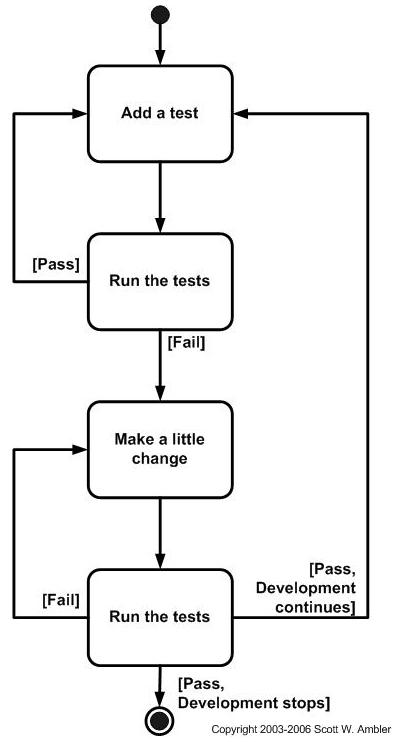
\includegraphics[scale=0.8]{TFD.png}

\section{Benefits of TDD}

TDD enables you to take small steps when writing software. This is the most important thing of this concept. This practice is far more productive than attempting to code in large steps. For example, assume some new functional code have been added to code, compiled, and tested. Chances are important that your tests will be broken by defects that exist in the new code. It is much easier to find, and then fix, those defects if you've written two new lines of code than two thousand. The implication is that the faster your compiler and regression test suite, the more attractive it is to proceed in smaller and smaller steps. I generally prefer to add a few new lines of functional code, typically less than ten, before I recompile and rerun my tests.


\section{Karma}

Karma is a test runner for JavaScript that runs on Node.js. It is very well suited to testing any JavaScript projects. Using Karma to run tests using one of many popular JavaScript testing suites (Jasmine, QUnit, Mocha, etc.) and have those tests executed not only in the browsers of your choice, but also on any platform (desktop, phone, tablet.) Karma is highly configurable, integrates with popular continuous integration packages (Jenkins, Travis, and Semaphore) and has excellent plugin support. Karma is an Open Source distribution and actually in the version 1.0.

\begin{itemize}
\item Installation - Karma requires Node.js and the Node Package Manager (NPM). So we can install Karma with the simple command:

\textdollar{} npm install -g karma
\item Configuration - A configuration file have first to be created. Then Karma can do what you want. This configuration file can be a JavaScript or a CoffeeScript file. The configuration file can be created manually or generated step by step via the command line:

\textdollar{} karma init

In this way, the created configuration file is then as follows:

\begin{lstlisting}[caption=Karma configuration file ]
       module.exports = function(config) {  
           config.set({  
               //  root path location that will be used to resolve  
               //all relative paths in files and exclude sections,  
               //should be the root of your project  
               basePath: '../',  
         
               // files to include, ordered by dependencies  
               files: [  
               // include relevant Angular files and libs  
               'app/lib/angular/angular.js',  
               'test/lib/angular/angular-mocks.js',  
     
               // include js files  
               'app/js/app.js',  
     
               // include unit test specs  
               'test/unit/*.js'  
           ],  
           // files to exclude  
           exclude: [  
            'app/lib/angular/angular-loader.js',  
               'app/lib/angular/*.min.js',  
               'app/lib/angular/angular-scenario.js'  
           ],  
     
           // karma has its own autoWatch feature but  
           //Grunt watch can also do this  
           autoWatch: false,  
     
           // testing framework, be sure to install  
           //the karma plugin  
           frameworks: ['jasmine'],  
     
           // browsers to test against, be sure to install   
           //the correct karma browser launcher plugin  
           browsers: ['Chrome', 'PhantomJS', 'Firefox'],  
     
           // progress is the default reporter  
           reporters: ['progress'],  
     
           // map of preprocessors that is used mostly   
           //for plugins  
           preprocessors: {  
     
           },  
     
           // list of karma plugins  
           plugins: [  
               'karma-junit-reporter',  
               'karma-chrome-launcher',  
               'karma-firefox-launcher',  
               'karma-jasmine',  
               'karma-phantomjs-launcher'  
           ]  
       })  
   }  
\end{lstlisting}

\item Application - Karma is started on the console with the following command:

\textdollar{} karma start [path/to/config/file.js]

All tests are now performed and Karma wait for code changes. while tests succeed, Karma will automatically start another test run. In the case of faulty test the result will be show in the console. In this case karma waits for an update or correction of JavaScript code.
\end{itemize}

\section{PhantomJS}

PhantomJS (phantomjs.org) is a headless WebKit scriptable with JavaScript. The latest stable release is version 2.1. PhantomJS is an open source, and is distributed under the BSD license. PhantomJS is created and maintained by Ariya Hidayat, with the help of many contributors.

PhantomJS can be used for many purpurses:

\begin{itemize}
\item Headless web testing: PhantomJS allows the Lightning-fast testing without the browser!
\item Page automation: With the tool it is also possible to Access and manipulate web pages with the standard DOM API, or with any JavaScript library.
\item Screen capture. PhantomJS provides a way to Programmatically capture web contents, including CSS, SVG and Canvas.
\item Network monitoring. PhantomJS facilitates the Automate performance analysis, tracks page loading and exports it as standard HAR format.
\end{itemize}

Among those use cases some features are implemented in PhantomJS:

\begin{itemize}
\item Multiplatform. This webkit is available on major operating systems like Windows, Mac OS X, Linux, and other Unices.
\item It provides a Fast and native implementation of web standards: DOM, CSS, JavaScript, Canvas, and SVG.
\item Pure headless (no X11) on Linux is made available, ideal for continuous integration systems. PhantonJS runs also on Amazon EC2, Heroku, and Iron.io.
\item PhantomJS is easy to install: Download, unpack, and start having fun in just 5 minutes.
\end{itemize}

\section{Jasmine}

Jasmine is an open source Javascript Unit Test Framework. It is behavior-driven development framework for testing JavaScript code. It does not depend on any other JavaScript frameworks. It does not require a DOM. And it has a clean, obvious syntax so that you can easily write tests. Now we will see how this framework is structured. The main particularities of Jasmine are:

\begin{itemize}
\item test Suite has a hierarchical structure,
\item tests integrated as specification,
\item matchers, both built-in and custom,
\item Setup and Teardown,
\item Spies, a test double pattern.
\end{itemize}

\subsection{Suites}

A test suite represents a group of specifications. The global Jasmine function describe defines a test suite. This function takes two parameters: a string and a closure. The title or name for a spec suite is defined by the string. It is usually what is being tested. A block of code that will be implemented will be wrote in the function.

\begin{lstlisting}[caption=Suites example]
       'use strict';  
         
       describe('A specification suite for Controller: MainCtrl', function () {  
         
           ...  
         
       });  
\end{lstlisting}

\subsection{Specs}

The global jasmine function „it“ define specs. This function, like „describe“ takes a string and a function. The title of the spec is defined by the string and the function is the spec, or test. One or more expectations that verify the state of the code are contained in a spec. In Jasmine an expectation is an assertion. This assertion can be true or false. A passing spec is a spec with all true expectations. A falling spec is rather a spec with one or more false expectations. 

\begin{lstlisting}[caption=Specs example]
       describe('Controller: StackCtrl: describes an abstract data' +  
                'type that serves as a collection of elements', function () {  
            
           it('specEmpty: if this stack is empty; Returns "true"' +  
              ' only if this stack don t contains  items; "false" otherwise', function () {  
         
               scope.stack = [{ firstname: "Peter", lastName: "Schneider"}];  
               expect(scope.isEmpty()).toBe(false);  
               scope.stack = [];  
           expect(scope.isEmpty()).toBe(true);      
         
      });  
   });  
\end{lstlisting}

Because the „describe“ and „it“ are function, ana executable code necessary to implement the spec can be defined in these blocks. So variables declared in a describe are available to any it block inside the suite.

\subsection{Expectations}

The function „expect“ is necessary to build expectations. This function takes an argument called the actual and is chained with a matcher function, which takes the expected value. A boolean comparison between the actual and the expected value will be implemented by each matcher. This matcher should report to Jasmine if the expectation is true or false. Then Jasmine decides if the spec pass or fails. With a „not“ before calling the matcher any matcher can evaluate to a negative chaining. Here is a list of most used matchers:

\begin{itemize}
\item expect(fn).toThrow(e);
\item expect(instance).toBe(instance);
\item expect(mixed).toBeDefined();
\item expect(mixed).toBeFalsy();
\item expect(number).toBeGreaterThan(number);
\item expect(number).toBeLessThan(number);
\item expect(mixed).toBeNull();
\item expect(mixed).toBeTruthy();
\item expect(mixed).toBeUndefined();
\item expect(array).toContain(member);
\item expect(string).toContain(substring);
\item expect(mixed).toEqual(mixed);
\item expect(mixed).toMatch(pattern);
\end{itemize}

Negative matchers can be call as followed:

\begin{itemize}
\item expect(instance).not.toBe(instance);
\item expect(mixed).not.toBeDefined();
\item expect(mixed).not.toBeFalsy();
\end{itemize}

The fail function brings a spec to fail. A failure message or an Error object can be take as parameter.

Custom matching code can be defined using Jasmine. A custom matcher can be defined as a comparison function, which take an „actual“ value and an „expected“ value. Then the custom factory should be passed to Jasmine. The best practice to do that is to pass it in the „beforeEach“ and it will be in scope and available for all of the specs inside a given call to „describe“. Custom matchers are destroyed between specs. The name of the factory will be the name of the matcher exposed on the return value of the call to „expect“. This object has a custom matcher named “toBeGoofy”. 

\begin{lstlisting}[caption=Custom matchers]
function compare(actual, expected) {
    var result = {};
    result.pass = actual <
        expected;
    if (result.pass === false) {
        result.message = function() {
            return "Expected " +
                actual +
                " not to be less than " +
                expected;
        };
    } else {
        result.message =
            function() {
                return "";
            };
    }
    return result;
}
beforeEach(function() {
    jasmine.addMatchers({
        toBeLessThan: function() {
            return {
                compare: compare
            }
        }
    });
});

...

it('Custum matchers', function() {
    expect(2).toBeLessThan(3);
});
\end{lstlisting}

\subsection{Setup and Teardown}

Related specs can be grouped by the „describe“ function. The string parameter is for naming the collection of specs, and will be concatenated with specs to make a spec’s full name. This is usefull in finding specs in a large suite. specs can be read as full sentences in traditional BDD style, if they are good named in the test blocks. Any duplicated setup and teardown code can be implemented in the global „beforeEach“, „afterEach“, „beforeAll“ and „afterAll“ functions. The „beforeEach“ function is called in the „describe“ in which it is called once before each spec. The „afterEach“ function is used once after each spec.

\begin{lstlisting}[caption=Setup and Teardown]
describe('StackCtrl', function() {

    var scope;

    beforeEach(function() {

        scope = new StackCtrl();
        scope.stack = [{
            firstname: "Cedric",
            lastName: "Takongmo"
        }, {
            firstname: "Peter",
            lastName: "Schneider"
        }];

    });

    afterEach(function() {
        scope = null;
    });

    it('specIsEmpty', function() {

        expect(scope.isEmpty()).toBe(false);
        scope.stack = [];
        expect(scope.isEmpty()).toBe(true);

    });
    it('specPush', function() {
        Scope.push({
            firstname: "Teddy",
            lastName: "Ricardo"
        });…
    });

});
\end{lstlisting}

The Abbildung 4 represents an example for „beforeEach“ and „afterEach“. In this case a state will be give to the „scope“ object we want to test before each test. Jasmine calls the „beforeAll“ function only once before all the specs in the test suite are run, and the „afterAll“ after all specs finish. These functions can be used to speed up test suites with expensive setup and teardown. Through the „this“ keyword variables between a „beforeEach“, „it“, and „afterEach“ function can be shared. Each spec’s „beforeEach“/„it“/„ afterEach“ has the „this“ as the same empty object that is set back to empty for the next spec’s „beforeEach“/„it“/„ afterEach“.

\subsection{Spies}

Test double function called spies can be defined by Jasmine. Any function can be stub by a spy ,which can tracks call to it and all arguments. definition area of a spy ist he „describe“ and the „it“ block in which it is defined. The spy will be destroyed after each spec. Some important matcher after a spy action are:

\begin{itemize}
\item The „toHaveBeenCalled“ matcher will return true if the spy was called.
\item The „toHaveBeenCalledTimes“ matcher will pass if the spy was called the specified number of times.
\item The „toHaveBeenCalledWith“ matcher will return true if the argument list matches any of the recorded calls to the spy.
\end{itemize}

\begin{lstlisting}[caption=Spy usage]
describe("A spy", function() {
    var foo, bar = null;

    beforeEach(function() {
        foo = {
            setBar: function(value) {
                bar = value;
            }
        };

        spyOn(foo, 'setBar');

        foo.setBar(123);
        foo.setBar(456, 'another param');
    });

    it("tracks that the spy was called", function() {
        expect(foo.setBar).toHaveBeenCalled();
    });

    it("tracks all the arguments of its calls", function() {
        expect(foo.setBar).toHaveBeenCalledWith(123);
        expect(foo.setBar).toHaveBeenCalledWith(456,
            'another param');
    });

    it("stops all execution on a function", function() {
        expect(bar).toBeNull();
    });
});
\end{lstlisting}

More others functions can be call by chaining the spy with:

\begin{itemize}
\item and.callThrough: the spy will still track all calls to it but in addition it will delegate to the actual implementation.
\item and.returnValue: all calls to the function will return a specific value.
\item and.callFake: all calls to the spy will delegate to the supplied function.
\item and.throwError: all calls to the spy will throw the specified value as an error.
\item and.stub: the original stubbing behavior can be returned at any time.
\end{itemize}

\section{Karma-coverage}

Karma-coverage is a npm peer dependency to generate test report using the „Istanbul“ library. This plugin can be simply installed by the command:

\textdollar{} npm install karma karma-coverage --save-dev

Then the developper can configurate the plugin using the karma.conf.je file. The Abbildung 7 shows how to configurate a karma-coverage plugin after install it to genarate Test reports.

\begin{lstlisting}[caption=Karma-coverage configuration's file]
// karma.conf.js  
module.exports = function(config) {
    config.set({
        files: [
            'src/**/*.js',
            'test/**/*.js'
        ],
        reporters: ['progress', 'coverage'],
        preprocessors: {
            'src/**/*.js': ['coverage']
        },
        coverageReporter: {
            // specify a common output directory  
            dir: 'build/reports/coverage',
            reporters: [
                // reporters not supporting the `file` property  
                {
                    type: 'html',
                    subdir: 'report-html'
                }, {
                    type: 'lcov',
                    subdir: 'report-lcov'
                },
                // reporters supporting the `file` property, use `subdir` to directly  
                // output them in the `dir` directory  
                {
                    type: 'cobertura',
                    subdir: '.',
                    file: 'cobertura.txt'
                }, {
                    type: 'lcovonly',
                    subdir: '.',
                    file: 'report-lcovonly.txt'
                }, {
                    type: 'teamcity',
                    subdir: '.',
                    file: 'teamcity.txt'
                }, {
                    type: 'text',
                    subdir: '.',
                    file: 'text.txt'
                }, {
                    type: 'text-summary',
                    subdir: '.',
                    file: 'text-summary.txt'
                },
            ]
        }
    });
};
\end{lstlisting}

\section{TDD - Best Practices}
In this part some of the best practices to be followed in TDD projects are presented:

\begin{itemize}
\item Avoid functional complexity
\item Focus on what you need to achieve
\item Maintain code austerity: Ensure your code has just enough meat to satisfy your test case
\item Test repeatedly
\item Maintain code sanctity
\item Application knowledge
\item Know when to use TDD
\end{itemize}

\section{Summary}


\begin{thebibliography}{9}

\bibitem{When2016} When do developers use JavaScript and why? - Quora. [Internet]. [cited 2016 Jul 20]. Available from:
\newblock {\em https://www.quora.com/When-do-developers-use-JavaScript-and-why}

\bibitem{Howt2016} How to define code quality - Quora. [Internet]. [cited 2016 Jul 20]. Available from:
\newblock {\em https://www.quora.com/How-do-you-define-code-quality}

\bibitem{Kent2003} Kent Beck
\newblock 2003.
\newblock {\em Test Driven Development: By Example}, 1st Edition.
\newblock Addison Wesley, Boston, MA.

\bibitem{Davi2003} David Astels
\newblock 2003.
\newblock {\em Test-Driven Development: A Practical Guide: A Practical Guide}, 1st Edition.
\newblock Pearson Education, Upper Saddle River, NJ.

\bibitem{Maxg2013} Max Guernsey III 
\newblock 2013.
\newblock {\em Test-Driven Database Development: Unlocking Agility (Net Objectives Lean-Agile Series)}, 1st Edition.
\newblock Pearson Education, USA.

\bibitem{Gojk2011} Gojko Adzic
\newblock 2011.
\newblock {\em Specification by Example: How Successful Teams Deliver the Right Software}, 1st Edition.
\newblock Manning Publications Co., Shelter Island, NJ.

\bibitem{Intr2013} Introduction to Test Driven Development (TDD). [Internet]. Ambysoft Inc. 2013 [cited 2016 Jul 20]. Available from: \newblock {\em http://agiledata.org/essays/tdd.html\#PartingThoughts}

\bibitem{Karm2013} Karma - a Javascript Test Runner. [Internet]. Michael G Bielski. 2013 [cited 2016 Jul 20]. Available from:
\newblock {\em http://www.methodsandtools.com/tools/karma.php}

\bibitem{Java2013} JavaScript Tests mit Karma schnell an den Start bringen - Mayflower Blog. [Internet]. Norbert Schmidt. 2013 [cited 2016 Jul 20]. Available from:
\newblock {\em https://blog.mayflower.de/4333-Karma-Testrunner-Einfuehrung.html}

\bibitem{phan2016} phantomjs/README.md at master · ariya/phantomjs [Internet]. Ariya Hidayat. 01.2016 [cited 2016 Jul 20]. Available from:
\newblock {\em https://github.com/ariya/phantomjs}

\bibitem{cust2016} custom\_matcher.js [Internet]. Pivotal Labs. 2016 [cited 2016 Jul 20]. Available from:
\newblock {\em http://jasmine.github.io/edge/custom\_matcher.html}

\bibitem{intr2016} introduction.js [Internet]. Pivotal Labs. 2016 [cited 2016 Jul 20]. Available from:
\newblock {\em http://jasmine.github.io/2.0/introduction.html\#section-Spies}

\bibitem{KarmCo2016} Karma-runner/karma-coverage: A Karma plugin. Generate code coverage. [Internet]. Friedel Ziegelmayer. 07.2016 [cited 2016 Jul 20]. Available from:
\newblock {\em https://github.com/karma-runner/karma-coverage}

\end{thebibliography}

\end{document}
\grid
\grid
\grid
